\chapter[On-Board Science Data Quality Analysis using Anomaly Detection for ASTHROS]{On-Board Science Data Quality Analysis using Anomaly Detection for ASTHROS}
\section{Abstract}
ASTHROS (Astrophysics Stratospheric Telescope for High Spectral Resolution Observations at Submillimeter-wavelengths) is a high-altitude balloon mission utilizing an array of sixteen spectrometers to create high spatial resolution 3D maps of ionized nitrogen gas in galactic and extragalactic star-forming regions.
During data collection, we utilize on-the-fly mapping, where the instrument continuously collects spectra while scanning over a target area.
After a sweep across the target, we take a calibration spectra to correct our science data.
These calibration spectra provide a baseline for how the instrument is operating at a given moment.
As we collect new calibration spectra, we can compare the current calibration with a series of past calibrations to determine if our system is producing anomalous spectra.
Some examples of anomalous spectra are changes in RFI spike frequency, location, or amplitudes, changes in the overall readout level, and changes in the shape of the spectra.
We compare statistical and data-driven methods for detecting these anomalies and evaluate their performance to determine the best fit for the ASTHROS readout system. For data-driven methods, we compare the latent space representation of our calibration spectra with past calibrations using models like Variational AutoEncoders (VAE) and Principal Component Analysis (PCA).
By comparing with a rolling window of past calibrations, we allow our system to change gradually while identifying sudden irregularities.
When spectra are labeled as anomalous, they are prioritized for review so that the ground operations team can analyze and address the issue.
On-board analysis is enabled by the readout system architecture which utilizes the RabbitMQ (RMQ) messaging networking.
RMQ allows us to modularly build our readout system and create additional functionality, such as on-board analysis, without making modifications to the operation pipeline. 


\section{Introduction}
ASTHROS (Astrophysics Stratospheric Telescope for High Spectral Resolution Observations at Submillimeter-wavelengths) is a high-altitude ballooning mission utilizing an array of sixteen spectrometers to create high spatial resolution 3D maps of ionized nitrogen gas in galactic and extragalactic star-forming regions \parencite{siles2020asthros}. 
On-the-fly (OTF) mapping will be employed during data collection where each spectrometer will continuously produce ON and OFF spectra as we scan across our target as show in in Figure \ref{spectra/fig:scan} \parencite{mangum2007fly}. 

\begin{figure}
    \centering
    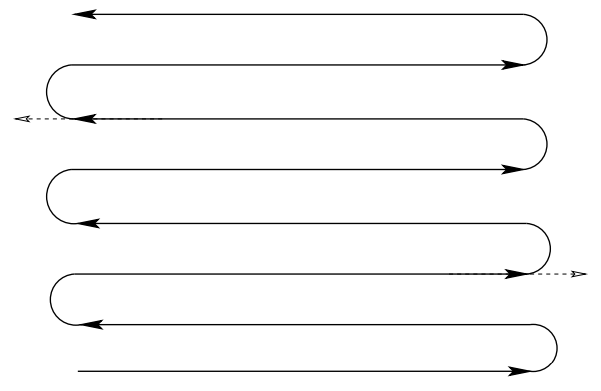
\includegraphics[width=0.5\linewidth]{figs/spectra/scan.png}
    \caption{An example scanning pattern for OTF mapping. ASTHROS will continuously produce ON spectra while scanning across the target and OFF spectra when observing a calibration source from \parencite{mangum2007fly}.}
    \label{spectra/fig:scan}
\end{figure}

Once data collection has started, our spectrometer array will continuously produce and timestamp spectra and save the raw time stream to itself and a separate storage device. 
The clocks of all the computers on board ASTHROS will be synchronized using a local NTP server such that the timestamps can be harmonized with pointing data from the gondola to label ON and OFF spectra \parencite{mills1991internet}.
After a sweep across the target, we will find spectra taken during the OFF segments and use them to evaluate our system's performance.
By generating an anomaly score for these calibrations, we can determine if our system is behaving differently than expected when compared to a series of past calibrations.

Currently, the methods for evaluating system performance are done on the ground by checking spectra manually as they come down.
This is an error-prone process as it is difficult to manually check each calibration spectrum for anomalies.
By implementing on-board anomaly detection, we can automate this process and prioritize analysis of anomalous spectra for review by the ground operations team.
This will allow us to quickly identify and address any issues with the system during flight to catch errors while within the window of opportunity to correct them instead of waiting until the end of the mission to find out that our data is unusable.
Even if the anomaly detection system is not perfect, any form of quantifiable measure of science data quality will be an improvement over the current manual process.


This paper will focus on the on-board analysis of our calibration spectra to detect anomalies in the system.
Section \ref{spectra/sec:system} will go over the system architecture for ASTHROS and how we can utilize RabbitMQ (RMQ) to enable on-board analysis.
After that, Section \ref{spectra/sec:methods} will discuss the methods we used to detect anomalies in our calibration spectra.
Then, in Section \ref{spectra/sec:data}, we will discuss the data we used to evaluate our methods and how we collected the data.
Section \ref{spectra/sec:results} will present the results of our analysis and conclude which method is the best fit for the ASTHROS readout system.
Finally, Section \ref{spectra/sec:future} will discuss future work for implementation on ASTHROS. 

\section{System Architecture}
\label{spectra/sec:system}
The ASTHROS readout system is composed of three main computers that respectively handle commanding the instrument, storing science data, and analyzing our telemetry and science data. 
Our goal with this readout system is to be able to collect and analyze data in real time so that any changes in detector behavior can be quickly identified and addressed during flight. 
To achieve this, we utilize RabbitMQ (RMQ) to create a modular system that can be easily expanded to include additional functionality by creating a standard protocol for Remote Procedure Calls (RPC) and Publish/Subscribe (Pub/Sub) messaging \parencite{dobbelaere2017kafkaversusrabbitmq}.
RMQ is a lightweight messaging broker based communications system used to seamlessly create a network of computers that are able to share status and commands between multiple concurrent processes \parencite{thompson2024architecture}.

\begin{figure}
    \centering
    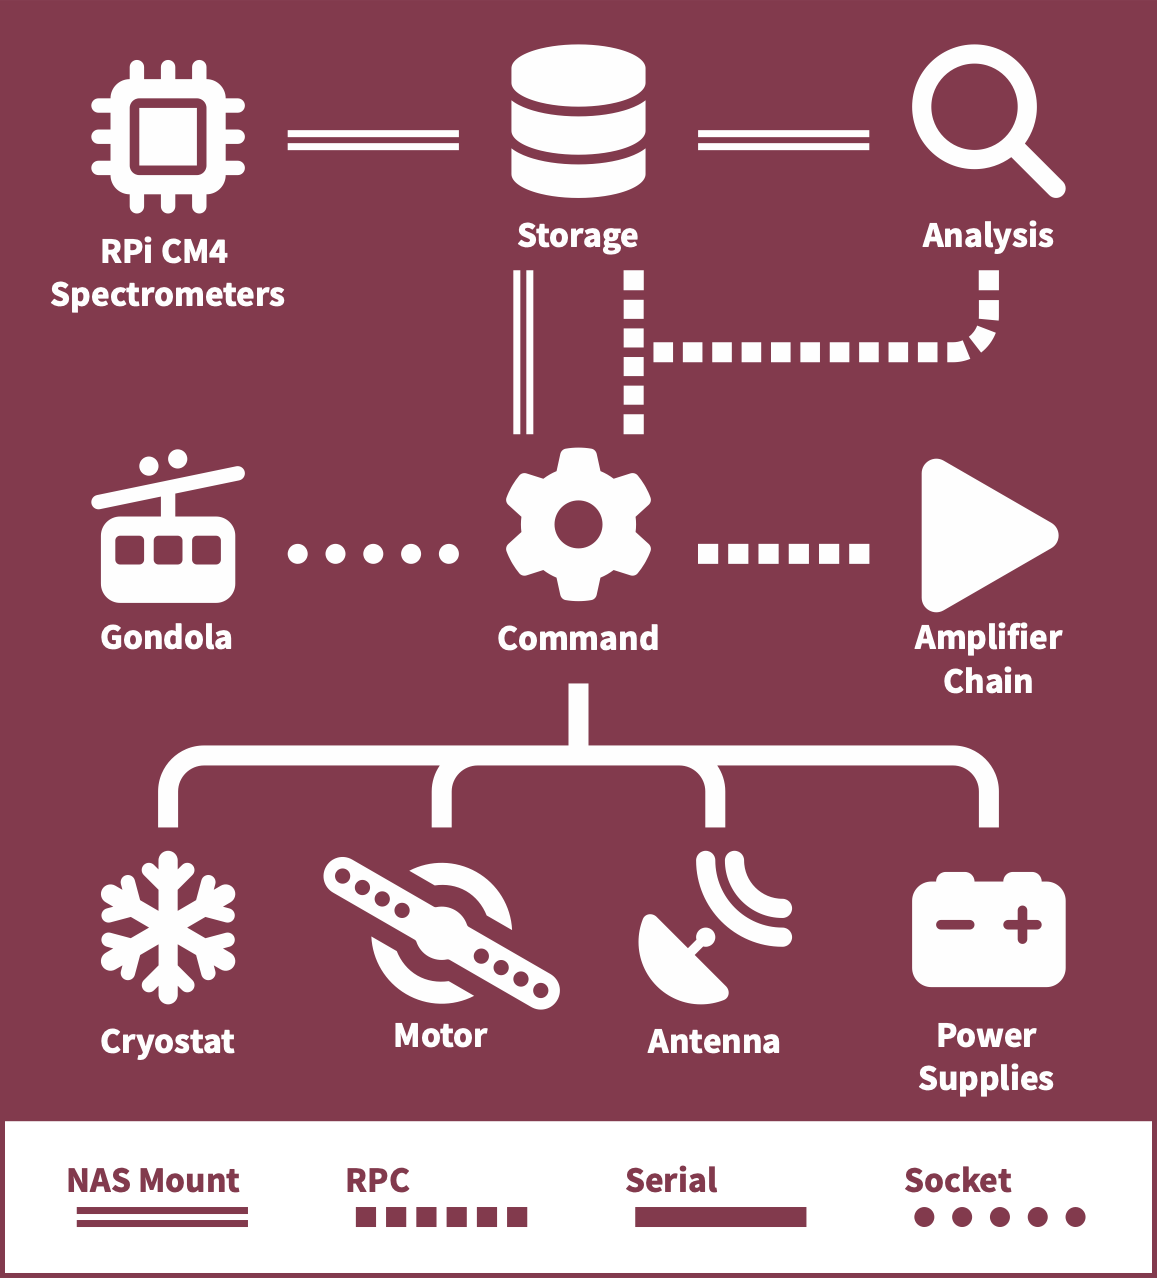
\includegraphics[width=0.5\linewidth]{figs/spectra/system.png}
    \caption{A high level overview of the ASTHROS Readout Network System Architecture showing the Command, Storage, and Analysis computers. The Command computer is responsible for sending commands to other processes and receiving status updates from the various publishers on the RMQ network. The Storage computer is responsible for storing all science data and telemetry data collected during the flight. The Analysis computer is responsible for analyzing the science data collected during the flight. The overview also shows some of the various subsystems and how they're connected in the network.}
    \label{spectra/fig:system}
\end{figure}

The core of ASTHROS's readout are three systems: the Command, Storage, and Analysis computers as shown in Figure \ref{spectra/fig:system} \parencite{horton2024readout}.
The Command computer is responsible for sending commands to other processes and receiving status updates from the various publishers on the RMQ network. 
This computer also manages telemetry through a connection to the gondola. 
Key system devices, such as the power supplies and the antenna, are connected directly to this computer via serial connections to allow for real-time monitoring and control.
Despite being physically on the same computer, control of each of these subsystems is handled by separate processes that communicate with the Central process through RMQ.
This allows any of these processes to be moved to a different computer or replaced with a new process without changing the overall system architecture.
As most of the systems are located on the Command computer, we host the RMQ broker on this computer to minimize latency and reduce the number of network hops between the Command computer and the other systems.

The Storage computer is responsible for storing all science data and telemetry data collected during the flight.
This computer is a custom-built rugged Network Attached Storage (NAS) that is able to store all the data collected during the flight.
This NAS houses 4 Solid State Drives in a RAID 10 configuration \parencite{chen1994raid}.
Other computers on the network, such as the Command computer and the Analysis computer, are able to mount the storage computer as a network drive to read and write data.
Additionally, this storage computer has two managed network switches that allow for networking to every system on ASTHROS.
Our spectrometers, controlled by Raspberry Pi CM4s, are connected to this computer via Ethernet and are able to store their data locally on their own Solid State Drives and send a copy to the storage computer.
We do this for redundancy in case the storage computer fails during flight.

Finally, we have the Analysis computer which is responsible for analyzing the science data collected during the flight. 
This computer has the critical task of analyzing the calibration spectra to determine if the system is behaving as expected by measuring data quality. 
The methods described in this paper are run on this computer and are able to communicate with the Command computer to prioritize analysis of anomalous spectra via telemetry.
Like other computers on the network, the Analysis computer is able to mount the storage computer as a network drive to read and write data.
Using RMQ, the analysis computer is able to listen to the status exchange for pointing updates from the gondola.
If the pointing data indicates that the telescope is observing a calibration source, the Analysis computer will pull the most recent calibration spectra from the storage computer and compare it to a series of past calibrations to determine if the system is behaving as expected.
In addition to it's primary function of analyzing science data, the Analysis computer is also able to run additional processes to prepare data for the science team. 
It does this by time harmonizing the science data with the pointing data from the gondola to label each spectra with the correct pointing information so that it may be used for mapping. 

Apart from the main three computers, the ASTHROS readout system also consists of a set of Raspberry Pi Compute Module 4s (CM4s) that control the spectrometers and a set of Arduino Nano Every microcontrollers that control the amplifier chains. 
Both of these are configured to communicate over the RMQ network for Command and Control and produce status updates over the Status Exchange. 
The CM4s are responsible for controlling the spectrometers and collecting the raw time stream data from the spectrometers \parencite{mohammed2024digital}.
The Arduinos are responsible for controlling the amplifier chains to adjust attenuation values for our variable attenuators \parencite{Ricardo}.

\section{Methods}
\label{spectra/sec:methods}
Anomaly detection, also known as outlier detection, is a way of finding out-of-distribution data points in a dataset \parencite{kerner2022domain}.
This works by comparing a data point to typical examples from the dataset and determining if the data point is significantly different from the rest of the data.
Because of the nature of anomalies, we can't use traditional supervised learning methods to detect them as we don't have labeled examples of what an anomaly looks like \parencite{horton2021integrating}.
In other words, we don't fully know what we don't know and, instead of training our system on known issues, we need to train our system to recognize when something is different from what it has seen before.
To do this, we need to use unsupervised learning methods that learn the underlying structure of our data and determine if a new data point is significantly different from the rest of the data.
Figure \ref{spectra/fig:examples} shows examples of the types of anomalies we have seen in past missions. 
Typically, these anomalies present themselves as changes in RFI spikes, the shape of the readout spectra, or the overall readout bias level.

\begin{figure}
    \centering
    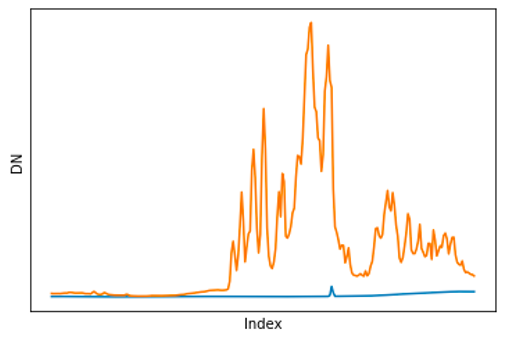
\includegraphics[width=0.3\linewidth]{figs/spectra/Anom1.png}
    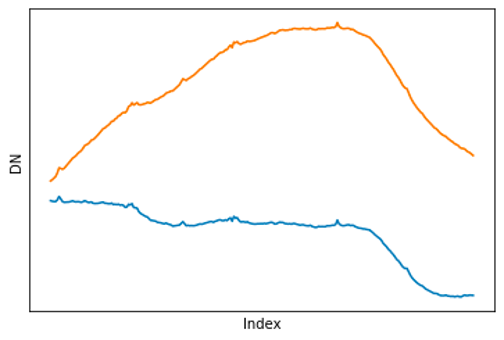
\includegraphics[width=0.3\linewidth]{figs/spectra/anom2.png}
    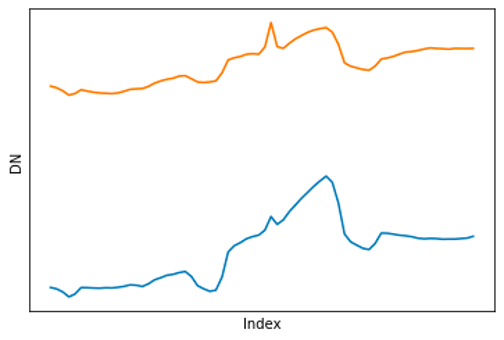
\includegraphics[width=0.3\linewidth]{figs/spectra/anom3.png}
    \caption{Examples of anomalous spectra from past missions. From left to right, we see changes in RFI spike shape and location, changes in the shape of the spectrum, and changes in the readout bias level.}
    \label{spectra/fig:examples}
\end{figure}

For this implementation, we focus on two methods for determining if a calibration spectrum is anomalous: Variational AutoEncoders (VAE) and Principal Component Analysis (PCA).
Both have their strengths and weaknesses and we compare their performance on the ASTHROS calibration spectra to determine which is the best fit for our system.

\subsection{Variational AutoEncoders}
VAEs are a class of AutoEncoders that learn the mean and variance of the latent space of the data \parencite{kingma2013auto}.
This is done by training the model to encode the input data into a lower dimensional space and then decode it back to the original input.
We selected VAEs for this task because they are able to learn the underlying structure of the data and generate new examples of the data by sampling from the latent space.
This is useful for anomaly detection as we can compare a new spectrum to the reconstructed spectrum to determine if it is significantly different from the rest of the data.
When a new spectrum is input into the VAE, the encoded and then decoded spectrum will be different from the original spectrum if the new spectrum is anomalous.

The architecture for our VAE is a simple feedforward neural network with multiple layers.
Our encoder consists of an input layer, a hidden layer, and two output layers for the mean and variance of the latent space.
The input layer has $8192$ nodes, one for each channel in our calibration spectra.
The hidden layer has $256$ nodes which feeds into our output layer which has $64$ nodes of mean and variance.
We re-parameterize the mean and variance to sample from the latent space and feed this into the decoder which has the same architecture hidden layer and input layers as the encoder but in reverse.
The output layer of the decoder has $8192$ nodes to reconstruct the original spectrum.

To train the VAE, we have to normalize our spectra to values between $0$ and $1$.
We then split our data into a training and testing set and train the VAE on the training set.
We then use the VAE to encode the testing set to it's latent space representation and decode it to produce a reconstructed version.

To generate an anomaly score from this method, we take a test spectrum, transform it using the VAE to it's latent space representation, and then decode the spectrum to produce a reconstructed version.
This reconstruction is imperfect as the VAE model is fit to our typical spectra.
We compare the reconstruction to our original spectrum to calculate error from the difference between the two specra.
This score can be used as a time series of anomaly scores to determine if a new spectrum is significantly different from the rest of the data. 
For flight, we will have to retrain the VAE on a subset of the data to account for changes in the system over time, making for more challenging flight integration.

\subsection{Principal Component Analysis}
PCA is a method that reduces the dimensionality of a dataset by finding the directions of maximum variance in the data \parencite{wold1987principal}.
This is done by finding the eigenvectors, called principal components, of the covariance matrix of the data and projecting the data onto these eigenvectors.
The first principal component is the direction of maximum variance in the data, the second principal component is the direction of maximum variance orthogonal to the first principal component, and so on.
Because our calibration spectra are high dimensional with $8192$ channels, we use PCA to reduce the dimensionality of our data to a lower dimensional space where we more easily compare the spectra.

To use PCA for anomaly detection, we first fit the PCA model to a series of past calibration spectra.
This can be done in two ways, fitting the PCA model to a subset of the spectra in an entire dataset and using a rolling window of past spectra to create unique fits for each additional spectrum. 
The first method can be used to determine if PCA is a good method for fitting to the dataset by seeing how many principal components are necessary to cover the variance of a typical spectrum. 
The second method can then be used in a real time setting to determine how a new spectrum compares to the recent history of previous spectra. 

To generate an anomaly score from this method, we take a test spectrum, transform it using the fit PCA model to it's latent space representation, and then inverse transform the spectrum to produce a reconstructed version. 
This reconstruction is imperfect as the PCA model is fit to our typical spectra.
We compare the reconstruction to our original spectrum to calculate the mean squared error from the difference between the two spectra. 
We use this value as our anomaly score as it provides a measure of how different a given spectrum is from previous spectra. 

\begin{figure}[b]
    \centering
    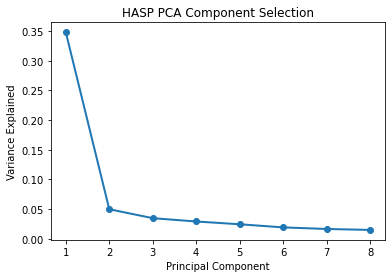
\includegraphics[width=0.49\linewidth]{figs/spectra/HASP_Elbow.png}
    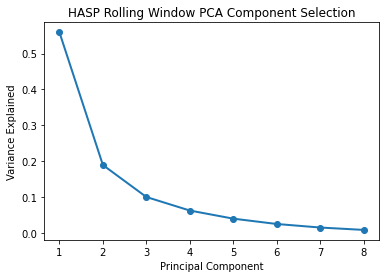
\includegraphics[width=0.49\linewidth]{figs/spectra/elbow.png}
    \caption{Elbow plots for the HASP dataset. Left shows the amount of variance each component accounts for in the entire dataset and the right shows the average variance amount when using a rolling window of 10 spectra.}
    \label{spectra/fig:elbows}
\end{figure}

\section{Data}
\label{spectra/sec:data}
The data for these tests are taken from two separate data collection instances. 
The first was a High-Altitude Student Platform (HASP) flight \parencite{guzik2008development} that tested one of our Pacific MicroCHIP Corp (PMCC) Spectrometers  \parencite{mohammed2024digital}.
A team of students at Arizona State University test flew a spare PMCC spectrometer to measure the deuterium to hydrogen ratio in the atmosphere \parencite{HADHR}.
Unfortunately, the spectrometer was not calibrated properly so many of the spectra were unusable for science. 
Additionally, due to the HASP payload's suite of student projects, we had many instances of changing RFI due to other instruments on board. 
Ironically, with all these problems, this dataset is an ideal candidate for testing the anomaly detection system as we are able to use it to evaluate good and bad spectra. 
This dataset consists of about 7,000 spectra of varied levels of noise. 

The second dataset was taken from one of our 100GHz integration tests with a flight calibrated spectrometer. 
This data is extremely stable and provides us an ideal baseline for what we expect to see during flight.
Despite being an extremely clean dataset of over 20,000 spectra, there are instances of RFI in the data that can be used to demonstrate the real time data quality assessment of the spectra. 

\begin{figure}
    \centering
    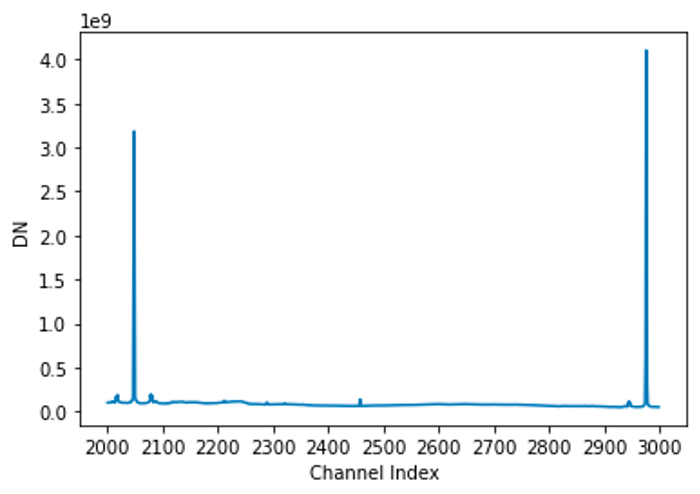
\includegraphics[width=0.49\linewidth]{figs/spectra/hasp1.png}
    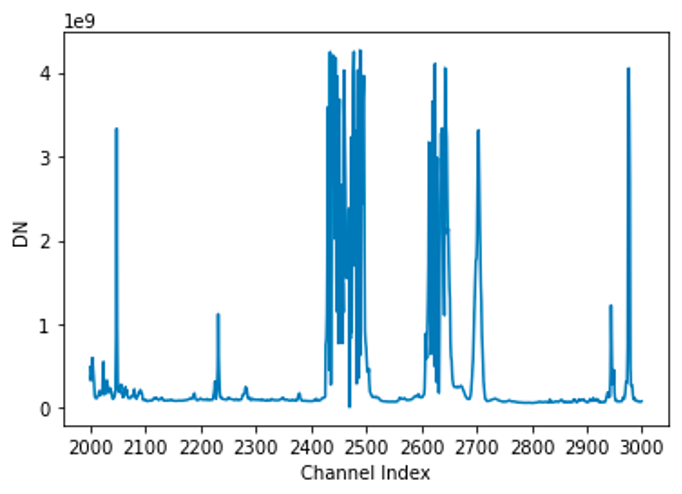
\includegraphics[width=0.49\linewidth]{figs/spectra/hasp2.png}
    \caption{Examples of spectra with the lowest (left) and highest (right) anomaly scores from the HASP dataset when using the PCA method to fit the entire HASP dataset.}
    \label{spectra/fig:hasp}
\end{figure}

One limitation of this dataset is that there aren't examples of changes in the baseline shape or bias readout level. 
These changes are rare and typically caused by physical changes in the instrument's hardware. 
In order to account for these, we would need to inject simulated anomalies in the data.
This is outside the scope of this work but will be discussed in Section \ref{spectra/sec:future}.

\section{Results and Conclusions}
\label{spectra/sec:results}
\begin{figure}[b]
    \centering
    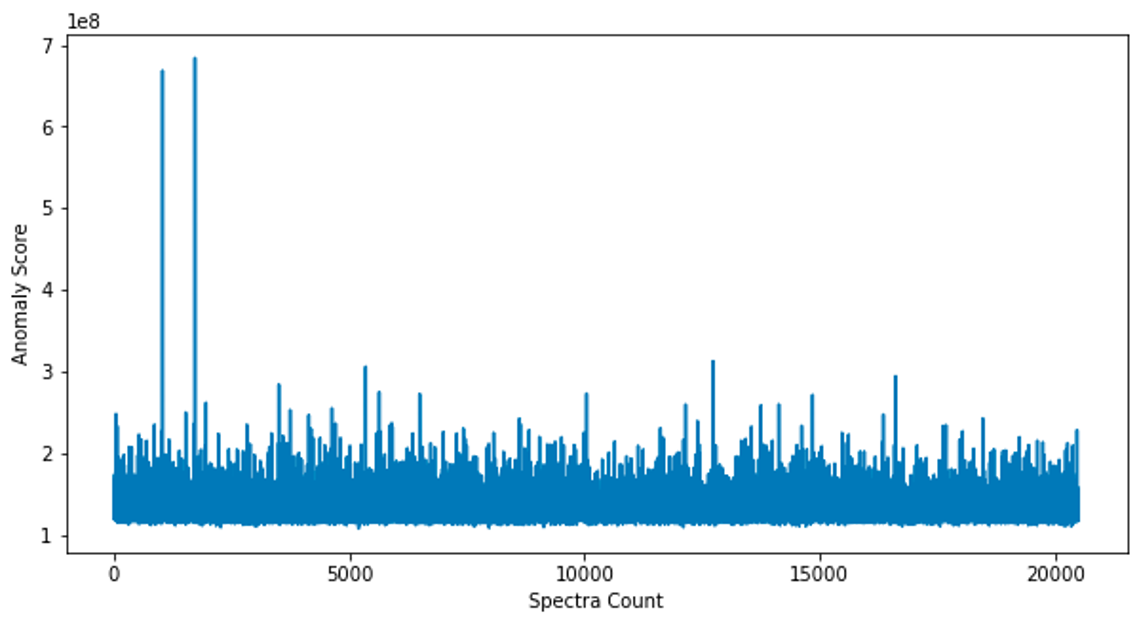
\includegraphics[width=0.5\linewidth]{figs/spectra/asthros_timeseries.png}
    \caption{A time series of anomaly scores using the PCA method for the 100GHz integration test data. Two large spikes are visible in the data indicating large changes between a spectrum and the previous spectra in the rolling window.}
    \label{spectra/fig:timeseries}
\end{figure}

Both datasets are unlabeled, which makes measuring accuracy difficult so we have to use more qualitative methods to compare the two.
The end use case of this method is to provide a trackable metric that the operations team can use to monitor data quality.
While accuracy is certainly important, any method that is able to enhance the manual monitoring process is sufficient. 
As such, we compare the methods based on their ability to be implemented into the ASTHROS System Architecture and how well the anomaly score metric tracks with manual monitoring of the time series of spectra over time. 
Additionally, we can compare the least and most anomalous spectra form the system to what sorts of anomalies produce high anomaly scores. 

With both datasets, the large number of features in the $8192$ channels, made it difficult for the VAE to learn the latent space for the spectra. 
Even after we managed to get it to behave properly, it became apparent that this method wouldn't adapt well for a rolling window of previous spectra. 
We would have to retrain the system on the fly to ensure that it adapted to gradual changes in instrument behavior.
With more refining and tests with domain adaptation, we may be able to revisit this method but, due to the overhead of having to retrain and the overall complexity of the system, we opted to focus on more adaptable methods. 


PCA was an ideal method for this use case. 
We began with the HASP dataset to see how the method would be able to rank spectra from least to most anomalous.
We first fit all of the $7000$ spectra with PCA to determine the number of components that would be optimal for comparison.
Most of the variances was captured with the first two principal components but, we opted to use five components as the variance increases when we're only looking at a portion of the dataset as shown in Figure \ref{spectra/fig:elbows}.
Using these number of components, we calculate the anomaly score for all of the spectra in the dataset to review the least and most anomalous spectra. 
See Figure \ref{spectra/fig:hasp} for the least and most anomalous spectra in the dataset. 
We've zoomed into a range of indices that were heavily affected by RFI, likely from another instrument. 
As expected, the least anomalous spectra look relatively clean and the most anomalous spectra are all very noisy. 

\begin{figure}[t]
    \centering
    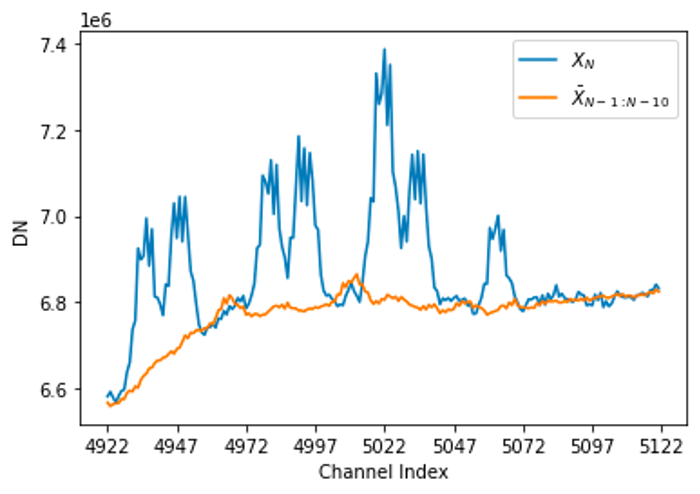
\includegraphics[width=0.49\linewidth]{figs/spectra/pca1.png}
    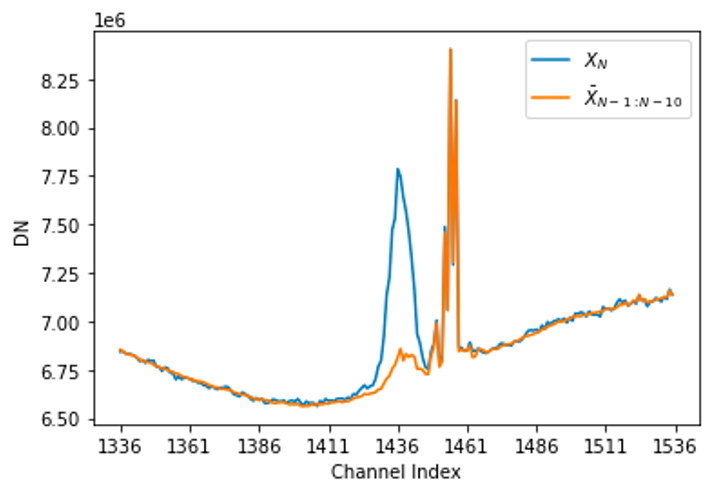
\includegraphics[width=0.49\linewidth]{figs/spectra/pca2.png}
    \caption{Examples from the 100GHz integration test data showing the spectra at the time of the two spikes in Figure \ref{spectra/fig:timeseries}. The blue line shows the spectra that has the high anomaly score and the orange line shows the average spectrum from the past 10 spectra. These spectra were highlighted due to the PCA method's inability to recreate the features shown in the new spectra when trained on the rolling window of previous spectra.}
    \label{spectra/fig:100ghz}
\end{figure}

On the cleaner 100GHz dataset, the method truly shined.
Using the same rolling window of 10 spectra and 5 principal components, we were able to produce a time series of anomaly scores for all 20,000 spectra as shown in Figure \ref{spectra/fig:timeseries}.
These values on their own don't provide much information but, when compared with other values across the dataset, we are able to pick out instances where our anomaly scores spiked. 
In the time series, there are two major spikes in the time series and a handful of smaller spikes throughout the test. 
We looked into these larger spikes in anomaly score and, they corresponded with spectrum that had changes in their RFI spikes.
Figure \ref{spectra/fig:100ghz} shows the affected channels of these anomalous spectra by overlapping them with the average of the previous 10 spectra. 
As shown in both examples, the new spectra has an increase in RFI that is different from the most recent spectra. 
On the other hand, the least anomalous spectra all closely match their predecessors. 
Of the tested methods, PCA has shown the most promise for implementation into the ASTHROS Readout System. 

\section{Future Work}
\label{spectra/sec:future}
The PCA method tested in this paper is currently being implemented onto the ASTHROS Readout Systems to test it in operations during ASTHROS's flight in 2024. 
The method will run on the analysis computer and integrate with the rest of the ASTHROS network to provide real-time data quality status messages over the RMQ status exchange.
During integration testing, the PCA method will be tested to ensure that it can handle the data rates and data sizes that will be produced during the flight. 

While the VAE method was less suitable for our use case, with more fine-tuning and optimization for the rolling window of past spectra, it could be a viable method for detecting anomalies in the future.
There are other methods, such as a Gaussian Mixture Model (GMM) or a Hidden Markov Model (HMM), that could be tested in the future to see if they are more suitable for our use case as well.

A limitation of our datasets are the lack of changes in shape of the spectrum or changes in bias level. 
In the future, we will make a simulator to inject these anomalies into our datasets to further test these methods. 
Additionally, with the flight of ASTHROS, we will have real calibration data to test everything on and reassess how we can improve our methods after using them for operations.